\documentclass{beamer}
\usepackage[utf8]{inputenc}
\usepackage[T1]{fontenc}
\usepackage{mathabx}
\usepackage{mathpazo}
\usepackage{eulervm}
\usepackage{natbib}
\usepackage{enumerate}
\usepackage{mathrsfs}

\usetheme{Madrid}
\usefonttheme{structurebold}
\usecolortheme{dove}
\title{VE401 RC Week3}
\author{Wang Yangyang}
\date{2022 Spring}
\institute{UM-SJTU JI}
\setbeamersize{text margin left = 20pt, text margin right = 20pt}

\AtEndDocument{\begin{frame}{End}
                  Credit to Zhanpeng Zhou (TA of SP21)
                  
                  Credit to Fan Zhang (TA of SU21)
                  
                  Credit to Jiawen Fan (TA of SP21)
                  
                  Credit to Zhenghao Gu (TA of SP20)
               \end{frame}
                }
                
\definecolor{antiquefuchsia}{rgb}{0.57, 0.36, 0.51}
\newcommand{\bb}[1]{\textcolor{antiquefuchsia}{\textbf{\textit{#1}}}}

\begin{document}
\maketitle

\begin{frame}
\frametitle{Outline}
\tableofcontents
\end{frame}

%\AtBeginSection[ ]
%{
%\begin{frame}{Outline for \secname}
%	\tableofcontents[currentsection, hideothersubsections, %sectionstyle=show/show]
%\end{frame}
%}

\AtBeginSubsection[]{
  \frame<beamer>{ 
    \frametitle{Outline}   
    \tableofcontents[currentsection,currentsubsection] 
  }
}


\section{Discrete Random Variables}
\subsection{Random Variables, PDF and CDF}
\begin{frame}{Random Variables}
\begin{block}{Assumption}
\begin{itemize}
\item We distinguish between 
\begin{itemize}
\item \bb{discrete random variables}, defined as having a countable range in $\mathbb{R}$
\item \bb{continuous random variables}, defined as having range equal to $\mathbb{R}$.
\end{itemize}
\item We assume that a random variable comes with a \bb{probability density} function that allows the calculation of probabilities directly, without recourse to the probability space.
\end{itemize}
\end{block}
\end{frame}

\begin{frame}{Discrete Random Variables and PDF}
\begin{block}{Definition}
Let $S$ be a sample space and $\Omega$ a countable subset of $\mathbb{R}$. A 
\bb{discrete random variable} is a map
$$
X: S \rightarrow \Omega
$$
together with a function
$$
f_{X}: \Omega \rightarrow \mathbb{R}
$$
having the properties that
\begin{itemize}
\item $f_{X}(x) \geq 0$ for all $x \in \Omega$ and
\item $\sum_{x \in \Omega} f_{X}(x)=1$.
\end{itemize}

\end{block}
The function $f_{X}$ is called the \bb{probability density function} or \bb{probability distribution} of $X$.

A \bb{random variable} is given by the pair $\left(X, f_{X}\right)$.
\end{frame}

\begin{frame}{Cumulative Density Function}
\begin{block}{Definition}
The cumulative distribution function of a random variable is defined as
$$
F_{X}: \mathbb{R} \rightarrow \mathbb{R}, \quad F_{X}(x):=P[X \leq x]
$$
For a discrete random variable,
$$
F_{X}(x)=\sum_{y \leq x} f_{X}(y)
$$
\end{block}

\end{frame}

\subsection{Expectation, Variance and Moments}
\begin{frame}{Expectation}
\begin{block}{Definition}
Let $\left(X, f_{X}\right)$ be a discrete random variable. Then the expected value or expectation of $X$ is
$$
\mathrm{E}[X]:=\sum_{x \in \Omega} x \cdot f_{X}(x)
$$
provided that the sum on the right converges absolutely.
\end{block}
We often write $\mu_{X}$ or simply $\mu$ for the expectation.
\begin{block}{Lemma}
Let $\left(X, f_{X}\right)$ be a discrete random variable and $\varphi: \Omega \rightarrow \mathbb{R}$ some function. Then the expected value of $\varphi \circ X$ is
$$
\mathrm{E}[\varphi \circ X]=\sum_{x \in \Omega} \varphi(x) \cdot f_{X}(x)
$$
provided that the sum (series) on the right converges absolutely.
\end{block}
\end{frame}

\begin{frame}{Expectation}
\begin{block}{Properties}
\begin{itemize}
\item Linearity

The expected value operator (or expectation operator) $\mathrm{E}[\cdot]$ is linear in the sense that, for any random variables $X$ and $Y$, and a constant $a$,
$$
\begin{aligned}
\mathrm{E}[X+Y] &=\mathrm{E}[X]+\mathrm{E}[Y] \\
\mathrm{E}[a X] &=a \mathrm{E}[X]
\end{aligned}
$$
whenever the right-hand side is well-defined. 

Symbolically, for $N$ random variables $X_{i}$ and constants $a_{i}(1 \leq i \leq N)$, we have $\mathrm{E}\left[\sum_{i=1}^{N} a_{i} X_{i}\right]=\sum_{i=1}^{N} a_{i} \mathrm{E}\left[X_{i}\right]$

\item Non-Multiplicity

If $X_{1}, \ldots, X_{n}$ are \bb{independent} random variables with finite expectations then
$
\mathrm{E}\left[\prod_{i=1}^{n} X_{i}\right]=\prod_{i=1}^{n} \mathrm{E}\left[X_{i}\right]
$.

However, if $X_{1}, \ldots, X_{n}$ are \bb{not independent}, then $
\mathrm{E}\left[\prod_{i=1}^{n} X_{i}\right]\neq\prod_{i=1}^{n} \mathrm{E}\left[X_{i}\right]
$.
\end{itemize}
\end{block}
\end{frame}

\begin{frame}{Variance}
\begin{block}{Definition}
\bb{The variance} is defined by
$$
\sigma_{X}^{2}=\operatorname{Var}[X]:=\mathrm{E}\left[(X-\mathrm{E}[X])^{2}\right]
$$
which is defined as long as the right-hand side exists. 

\bb{The standard deviation} is $\sigma_{X}=\sqrt{\operatorname{Var}[X]}$.
\end{block}
While expectation can be seen as a measure of location, 

variance can be seen as a measure of dispersion.
\begin{block}{Useful Formula}
$$\begin{aligned}
\operatorname{Var}[X] &=\mathrm{E}\left[(X-\mathrm{E}[X])^{2}\right] \\
&=\mathrm{E}\left[X^{2}-2 \mathrm{E}[X] \cdot X+\mathrm{E}[X]^{2}\right] \\
&=\mathrm{E}\left[X^{2}\right]-\mathrm{E}[X]^{2}
\end{aligned}$$
\end{block}
\end{frame}

\begin{frame}{Variance}
\begin{block}{Properties}
\begin{itemize}
\item
Variance is non-negative. 
$
\operatorname{Var}(X) \geq 0
$
\item
Variance of a constant is zero. 
$
\operatorname{Var}(a)=0
$
\item
Variance is invariant with respect to constant added to all values of the variable. 
$
\operatorname{Var}(X+a)=\operatorname{Var}(X)
$
\item
If all values are scaled by a constant, the variance is scaled by the square of that constant. 
$
\operatorname{Var}(a X)=a^{2} \operatorname{Var}(X)
$
\item
The variance of a sum of two \bb{independent} random variables is given by
$$
\begin{aligned}
&\operatorname{Var}(a X+b Y)=a^{2} \operatorname{Var}(X)+b^{2} \operatorname{Var}(Y)\\
&\operatorname{Var}(a X-b Y)=a^{2} \operatorname{Var}(X)\bb{+}b^{2} \operatorname{Var}(Y)
\end{aligned}
$$
(If not independent, then covariance should be considered.)
\end{itemize}
\end{block}
\end{frame}

\begin{frame}{Variance}
\begin{block}{Example}
Prove $\operatorname{Var}[X+Y]=\operatorname{Var}[X-Y]=\operatorname{Var}[X]+\operatorname{Var}[Y]$ for two \bb{independent} random variables $X$, $Y$.
\end{block}
\pause
\begin{block}{Solution}
$$
\begin{aligned}
\operatorname{Var}[X+Y] &=\mathrm{E}\left[\left(X+Y-\left(\mu_{X}+\mu_{Y}\right)\right)^{2}\right] \\
&=\mathrm{E}\left[\left(X-\mu_{X}\right)^{2}\right]+\mathrm{E}\left[\left(Y-\mu_{Y}\right)^{2}\right]\\
&+2 \mathrm{E}\left[\left(X-\mu_{X}\right)\left(Y-\mu_{Y}\right)\right]
\end{aligned}
$$
If $X,Y$ are independent, $\mathrm{E}\left[\left(X-\mu_{X}\right)\left(Y-\mu_{Y}\right)\right]=\mathrm{E}[X-\mu_{X}]\mathrm{E}[Y-\mu_{Y}]=0\times 0=0$.
\end{block}
\end{frame}

\begin{frame}{Ordinary and Central Moments}
\begin{block}{Definition}
The $n^{\text {th }}$ (ordinary) \bb{moments} of a random variable $X$ is given by
$$\mathrm{E}\left[X^{n}\right], \quad n \in \mathbb{N} .$$

The $n^{\text {th }}$ \bb{central moments} of $X$ is given by
$$\mathrm{E}\left[\left(\frac{X-\mu}{\sigma}\right)^{n}\right], \quad \text{ where } n=3,4,5, \ldots$$
\end{block}
\end{frame}

\begin{frame}{Moment-Generating Function}
\begin{block}{Definition}
Let $\left(X, f_{X}\right)$ be a random variable and such that the sequence of moments $E\left[X^{n}\right], n \in \mathbb{N}$, exists. If the power series
$$
m_{X}(t):=\sum_{k=0}^{\infty} \frac{\mathrm{E}\left[X^{k}\right]}{k !} t^{k}
$$
has radius of convergence $\varepsilon>0$, the thereby defined function
$$
m_{X}(t):(-\varepsilon, \varepsilon) \rightarrow \mathbb{R}
$$
is called the \bb{moment-generating function} for $X$.
\end{block}
\end{frame}

\begin{frame}{Moment-Generating Function}
\begin{block}{Theorem}
Let $\varepsilon>0$ be given such that $\mathrm{E}\left[e^{t X}\right]$ exists and has a power series expansion in $t$ that converges for $|t|<\varepsilon$. Then the \bb{moment-generating function} exists and
$$
m_{X}(t)=\mathrm{E}\left[e^{t X}\right] \quad \text { for }|t|<\varepsilon
$$
Furthermore,
$$
\mathrm{E}\left[X^{k}\right]=\left.\frac{\mathrm{d}^{k} m_{X}(t)}{\mathrm{d} t^{k}}\right|_{t=0}
$$
We can hence calculate the moments of $X$ by differentiating the moment-generating function.
\end{block}
\end{frame}

\begin{frame}{Moment-Generating Function}
\begin{block}{Properties}
\begin{itemize}
\item $X$ is a random variable and $Y=a X+b, a, b \in \mathbb{R}$, then for every $t$ such that $m_{X}(a t)$ is finite,
$$
m_{Y}(t)=e^{b t} m_{X}(a t) .
$$
\item Suppose $X_{1}, \ldots, X_{n}$ are $n$ independent random variables, then for every value that $m_{X_{i}}(t)$ is finite for all $i=1, \ldots, n$,
$$
m_{X}(t)=\prod_{i=1}^{n} m_{X_{i}}(t), \quad X=X_{1}+\cdots+X_{n} .
$$
\end{itemize}
\end{block}
\end{frame}


\begin{frame}{Moment-Generating Function}
\begin{block}{Example}
Suppose that $X$ is a random variable with the moment-generating function
$$
m_{X}: \mathbb{R} \rightarrow \mathbb{R}, \quad m_{X}(t)=e^{t^{2}+3 t}
$$
Find the mean and variance of $X$.
\end{block}
\pause
\begin{block}{Solution}
We calculate
$$
m_{X}^{\prime}(t)=(2 t+3) e^{t^{2}+3 t}, \quad m_{X}^{\prime \prime}(t)=(2 t+3)^{2} e^{t^{2}+3 t}+2 e^{t^{2}+3 t}
$$
Therefore,
$$
\mu=m_{X}^{\prime}(0)=3, \quad \sigma^{2}=\mathrm{E}\left[X^{2}\right]-\mathrm{E}[X]^{2}=m_{X}^{\prime \prime}(0)-\mu^{2}=2
$$
\end{block}
\end{frame}

\section{Distributions of Discrete Random Variable}
\subsection{Bernoulli, Binomial Distribution}

\begin{frame}{Bernoulli Distribution}
\begin{block}{Definition}
A random variable $\left(X, f_{X}\right)$ has a \bb{Bernoulli distribution} with parameter $p, 0<p<1$ if the probability density function is defined by
$$
f_{X}:\{0,1\} \rightarrow \mathbb{R}, \quad f_{X}(x)= \begin{cases}1-p, & \text { if } x=0 \\ p, & \text { if } x=1\end{cases}
$$
\end{block}
\begin{block}{Interpretation}
Describe the probability of success $f_{X}(1)$ or failure $f_{X}(0)$ of a trial, given the probability of success is $p$.
\end{block}
\end{frame}

\begin{frame}{Bernoulli Distribution}
\begin{block}{Properties}
\begin{itemize}
\item Mean
$$
\mathrm{E}[X]=0 \cdot(1-p)+1 \cdot p=p
$$
\item Variance
$$
\operatorname{Var}[X]=\mathrm{E}\left[X^{2}\right]-\mathrm{E}[X]^{2}=p-p^{2}=p(1-p)
$$
\item M.G.F.
$$
m_{X}: \mathbb{R} \rightarrow \mathbb{R}, \quad m_{X}(t)=1-p+pe^{t} 
$$
\end{itemize}
\end{block}
\end{frame}

\begin{frame}{Binomial Distribution}
\begin{block}{Definition}
A random variable $\left(X, f_{X}\right)$ has a \bb{Binomial distribution} with parameter $n \in \mathbb{N} \backslash\{0\}$ and $p, 0<p<1$ if it has probability density function
$$
f_{X}:\{0, \ldots, n\} \rightarrow \mathbb{R}, \quad f_{X}(x)=\left(\begin{array}{l}
n \\
x
\end{array}\right) p^{x}(1-p)^{n-x}
$$
\end{block} 
\begin{block}{Interpretation}
$f_{X}(x)$ is the probability of obtaining $x$ successes in $n$ independent and identical Bernoulli trials with parameter $p$.
\end{block}
\end{frame}

\begin{frame}{Binomial Distribution}
\begin{block}{Properties}
\begin{itemize}
\item Mean
$$
\mathrm{E}[X]=\sum_{i=1}^{n} \mathrm{E}\left[X_{i}\right]=n p
$$
\item Variance
$$
\operatorname{Var}[X]=\sum_{i=1}^{n} \operatorname{Var}\left[X_{i}\right]=n p(1-p)
$$
\item M.G.F.
$$
m_{X}: \mathbb{R} \rightarrow \mathbb{R}, \quad m_{X}(t)=\mathrm{E}\left[e^{t X}\right]=\prod_{i=1}^{n} \mathrm{E}\left[e^{t X_{i}}\right]=\left(1-p+p e^{t}\right)^{n}
$$
\end{itemize}
\end{block}
\end{frame}


\subsection{Geometric, Pascal, Negative Binomial Distribution}
\begin{frame}{Geometric Distribution}
\begin{block}{Definition}
A random variable $\left(X, f_{X}\right)$ has \bb{Geometric distribution} with parameter $p, 0<p<1$ if the probability density function is given by
$$
f_{X}: \mathbb{N} \backslash\{0\} \rightarrow \mathbb{R}, \quad f_{X}(x)=(1-p)^{x-1} p .
$$
\end{block}
\begin{block}{Interpretation}
$f_{X}(x)$ is the probability of $x$ failures before the first success in the Bernoulli trials, given the probability of success for each trial is $p$.
\end{block}
\end{frame}

\begin{frame}{Geometric Distribution}
\begin{block}{Properties}
Let $q=1-p$,
\begin{itemize}
\item Mean
$$
\mathrm{E}[X]=\frac{1}{p}
$$
\item Variance
$$
\operatorname{Var}[X]=\frac{q}{p^{2}}
$$
\item M.G.F.
\begin{align*}
\begin{aligned}
&m_{X}:(-\infty,-\ln q)\rightarrow \mathbb{R}\\
&m_X(t)=\sum_{k=1}^{\infty} e^{t k} pq^{k-1}
=p e^{t} \sum_{k=1}^{\infty} (e^{t}q)^{k-1}=\frac{p e^{t} }{1-qe^{t}}
\end{aligned}
\end{align*}
The geometric series only converges if $e^{t}q<1$.
\end{itemize}
\end{block}
\end{frame}


\begin{frame}{Pascal Distribution}
\begin{block}{Definition}
A random variable $\left(X, f_{X}\right)$ has the \bb{Pascal distribution} with parameters $p, 0<p<1$ and $r \in \mathbb{N} \backslash\{0\}$ if the probability density function is given by
$$
f_{X}:\{r, r+1, \ldots\} \rightarrow \mathbb{R}, \quad f_{X}(x)=\left(\begin{array}{c}
x-1 \\
r-1
\end{array}\right) p^{r}(1-p)^{x-r}
$$
\end{block}
\begin{block}{Interpretation}
$f_{X}(x)$ is the probability of obtaining the $r$-th success in the $x$-th Bernoulli trial, given the probability of success for each trial is $p$.
\end{block}
\end{frame}

\begin{frame}{Pascal Distribution}
\begin{block}{Properties}
Let $q=1-p$,
\begin{itemize}
\item Mean
$$
\mathrm{E}[X]=\frac{r}{p}
$$
\item Variance
$$
\operatorname{Var}[X]=\frac{rq}{p^{2}}
$$
\item M.G.F.
$$
m_{X}:(-\infty,-\ln q) \rightarrow \mathbb{R}, \quad m_{X}(t)=\frac{\left(p e^{t}\right)^{r}}{\left(1-qe^{t}\right)^{r}}
$$
\end{itemize}
\end{block}
\end{frame}


\begin{frame}{Negative Binomial Distribution}
\begin{block}{Definition}
A random variable $\left(X, f_{X}\right)$ has the \bb{Negative Binomial distribution} with parameters $r$ and $p$ if the probability density function is given by
$$
f_{X}: \mathbb{N} \rightarrow \mathbb{R}, \quad f_{X}(x)=\left(\begin{array}{c}
x+r-1 \\
r-1
\end{array}\right) p^{r}(1-p)^{x}
$$
\end{block}
\begin{block}{Interpretation}
$f_{X}(x)$ is the probability of $x$ failures before first obtaining $r$ successes in Bernoulli trials, given the probability for each success is $p$.
\end{block}
\end{frame}

\begin{frame}{Negative Binomial Distribution}
\begin{block}{Properties}
Let $q=1-p$,
\begin{itemize}
\item Mean
$$
\mathrm{E}[X]=\frac{r p}{q}
$$
\item Variance
$$
\operatorname{Var}[X]=\frac{r p}{q^{2}}
$$
\item M.G.F.
$$
m_{X}:(-\infty,-\ln q) \rightarrow \mathbb{R}, \quad m_{X}(t)=\frac{p^{r}}{\left(1-q e^{t}\right)^{r}}
$$
\end{itemize}
\end{block}
\end{frame}

\subsection{Poisson Distribution}
\begin{frame}{Poisson Distribution}
\begin{block}{Definition}
A random variable $X$ has the \bb{Poisson distribution} with parameter $k>0$ if probability density function is given by
$$
f_{X}: \mathbb{N} \rightarrow \mathbb{R}, \quad f_{X}(x)=\frac{k^{x} e^{-k}}{x !}
$$
\end{block}
\begin{block}{Interpretation}
$f_{X}(x)$ is the probability of $x$ arrivals in the time interval $[0, t]$ with arrival rate $\lambda>0$, and $k=\lambda t$.

"...which describes the occurrence of events that occur at \bb{constant rate} and \bb{continuous environment}."
\end{block}
\end{frame}


\begin{frame}{Poisson Distribution}
\begin{block}{Interpretation}
\begin{itemize}
\item \bb{Continuous environment}. Not limited to time intervals, but also subregions of two- or three-dimensional regions or sublengths of a linear distance, and any regions that can be divided into arbitrarily small pieces.
\item \bb{Constant rate}. The probability of an occurrence during each very short interval (region) must be approximately proportional to the length (area, volume) of that interval (region).
\end{itemize}
\end{block}
\begin{block}{Example}
Poisson process can be used to model
\begin{itemize}
\item the number of particles that strike a certain target at a constant rate in a particular period;
\item the number of oocysts that occur in a water supply system given constant rate of occurrence per liter...
\end{itemize}
\end{block}
\end{frame}

\begin{frame}{Poisson Distribution}
\begin{block}{Properties}
\begin{itemize}
\item Mean
$$
\mathrm{E}[X]=k
$$
\item Variance
$$
\operatorname{Var}[X]=k
$$
\item M.G.F.
$$
m_{X}: \mathbb{R} \rightarrow \mathbb{R}, \quad m_{X}(t)=e^{k\left(e^{t}-1\right)}
$$
\end{itemize}
\end{block}
\begin{block}{Derivation}
\begin{align*}
m_{X}(t)=\mathrm{E}\left(e^{t X}\right)=\sum_{n=0}^{\infty} P(X=n) e^{t n}
=\sum_{n=0}^{\infty} \frac{\lambda^{n} e^{-\lambda}}{n !} e^{t n}\\ 
=e^{-\lambda} \sum_{n=0}^{\infty} \frac{\left(\lambda e^{t}\right)^{n}}{n !} 
=e^{-\lambda} e^{\lambda e^{t}} 
=e^{\lambda\left(e^{t}-1\right)}
\end{align*}
\end{block}
\end{frame}

\subsection{Summary for Common Distributions}
\begin{frame}{Connections}
\begin{columns}
\column{\dimexpr\paperwidth-30pt}
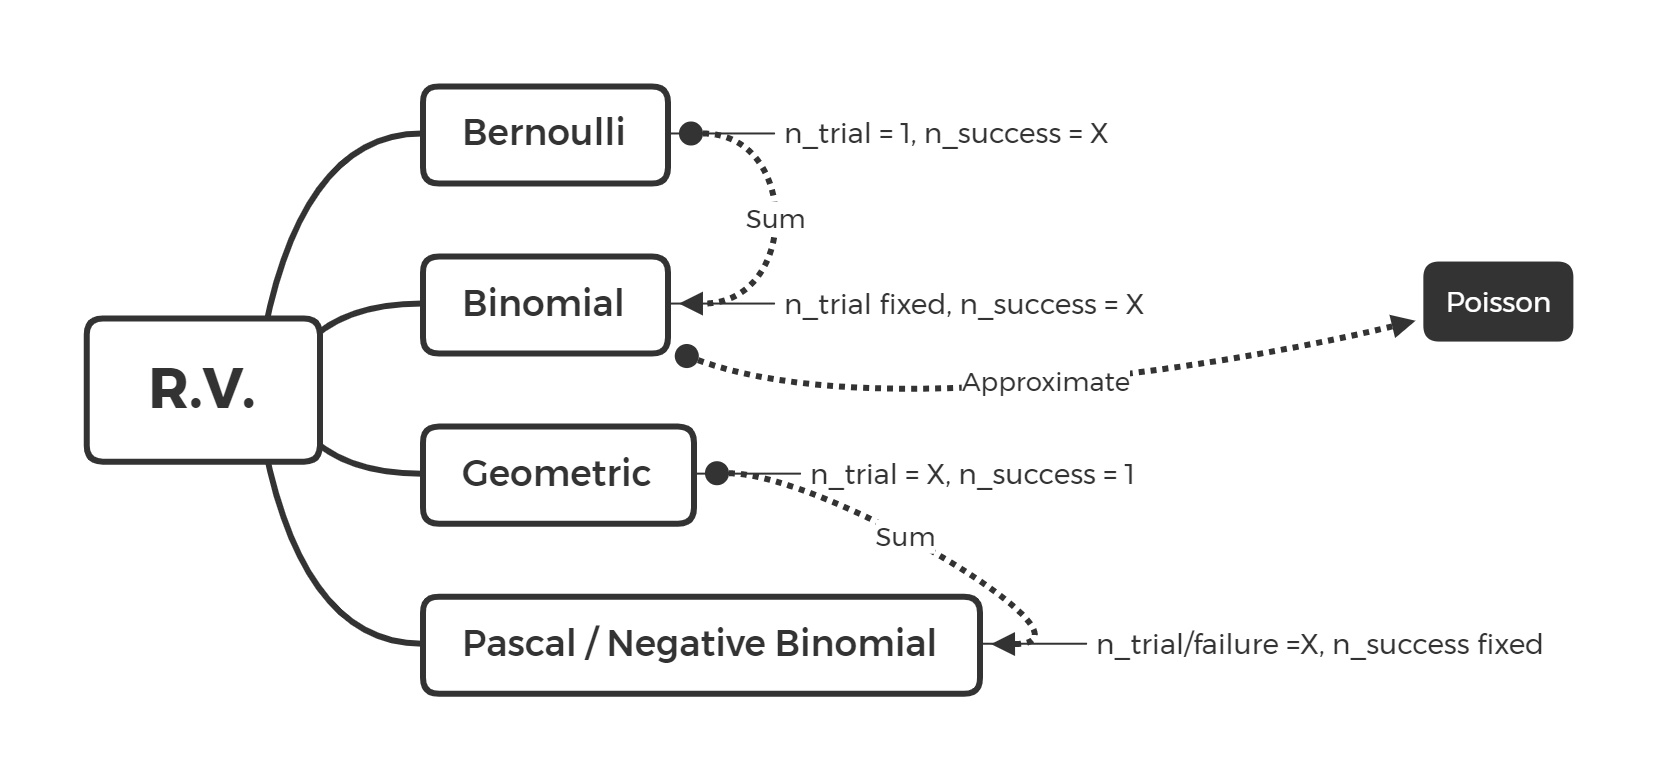
\includegraphics[scale=0.22]{Discrete.jpg}
\end{columns}
\end{frame}

\begin{frame}{Summations}
\begin{itemize}
\item Bernoulli $\rightarrow$ Binomial. $X_{1}, \ldots, X_{n}$ are independent random variables,
$$
X_{i} \sim \operatorname{Bernoulli}(p) \quad \Rightarrow \quad X=X_{1}+\cdots+X_{n} \sim \mathrm{B}(n, p) .
$$
\item Geometric $\rightarrow$ Pascal/Negative Binomial. $X_{1}, \ldots, X_{r}$ are independent random variables,
$$
X_{i} \sim \operatorname{Geom}(p) \quad \Rightarrow \quad X=X_{1}+\cdots+X_{r} \sim \operatorname{Pascal}(r, p) .
$$
\item Poisson $\rightarrow$ Poisson. $X_{1}, \ldots, X_{n}$ are independent random variables,
$$
X_{i} \sim \operatorname{Poisson}\left(k_{i}\right) \quad \Rightarrow \quad X=X_{1}+\cdots+X_{n} \sim \operatorname{Poisson}(k)
$$
where $k=k_{1}+\cdots+k_{n}$.
\end{itemize}
\end{frame}

\begin{frame}{Summations}
\begin{itemize}
\item Binomial $\rightarrow$ Binomial. $X_{1}, \ldots, X_{k}$ are independent random variables,
$$
X_{i} \sim B\left(n_{i}, p\right) \quad \Rightarrow \quad X=X_{1}+\cdots+X_{k} \sim B(n, p),
$$
where $n=n_{1}+\cdots+n_{k}$.

\item Negative Binomial $\rightarrow$ Negative Binomial. $X_{1}, \ldots, X_{n}$ are independent random variables,
$$
X_{i} \sim \operatorname{NB}\left(r_{i}, p\right) \quad \Rightarrow \quad X=X_{1}+\cdots+X_{n} \sim \operatorname{NB}(r, p),
$$
where $r=r_{1}+\cdots+r_{n}$.

\item Pascal $\rightarrow$ Pascal. $X_{1}, \ldots, X_{n}$ are independent random variables,
$$
X_{i} \sim \operatorname{Pascal}\left(r_{i}, p\right) \quad \Rightarrow \quad X=X_{1}+\cdots+X_{n} \sim \operatorname{Pascal}(r, p),
$$
where $r=r_{1}+\cdots+r_{n}$.
\end{itemize}
\end{frame}


\begin{frame}{Summations}
\begin{block}{Example}
Let $X$ be a discrete random variable following a \bb{Geometric distribution} with parameter $p=1 / 2$ and let $X_{1}, \ldots, X_{10}$ be a random sample of size 10 . Calculate the probability that the sample mean is no more than than $1.5$, i.e., find
$
P[\overline{X} \leq 1.5]
$.
\end{block}
\pause
\begin{block}{Solution}
We note that $X_{1}+\cdots+X_{10}$ follows a \bb{Pascal distribution} with $r=10$ and $p=1 / 2$.
Then
$$
\begin{aligned}
P[\overline{X}<1.5] &=P\left[X_{1}+\cdots+X_{10} \leq 10 \cdot 1.5\right]
=P\left[X_{1}+\cdots+X_{10} \leq 15\right] \\
&=\sum_{x=10}^{15}\left(\begin{array}{c}
x-1 \\
9
\end{array}\right) \frac{1}{2^{x}} =\frac{309}{2048}=0.15
\end{aligned}
$$
How about \bb{Negative Binomial} with $r=10$ and $p=1/2$?
\end{block}
\end{frame}

\begin{frame}{Closeness Between Poisson Distribution and Binomial Distribution}
\begin{block}{Theorem}
For $n \in \mathbb{N} \backslash\{0\}, 0<p<1$, suppose $f(x ; n, p)$ denotes the probability density function of \bb{Binomial distribution} with parameters $n$ and $p$, while $f(x ; k)$ denotes the probability density function of \bb{Poisson distribution} with parameter $k$. Let $\left\{p_{n}\right\}_{n=1}^{\infty}$ be a sequence of numbers between 0 and 1 such that
$$
\lim _{n \rightarrow \infty} n p_{n}=k
$$
then
$$
\lim _{n \rightarrow \infty} f\left(x ; n, p_{n}\right)=f(x ; k), \quad \text { for all } x=0,1, \ldots
$$
\end{block}
This means we can approximate the \bb{Binomial distribution} with \bb{Poisson distribution} when $n$ is large.
\end{frame}

\section{Continuous Random Variables}
\subsection{PDF, CDF and Location}
\begin{frame}{Continuous Random Variable: Def. and PDF}
\begin{block}{Definition}
Let $S$ be a sample space. A \bb{continuous random variable} is a map $X: S \rightarrow \mathbb{R}$ together with a function $f_{X}: \mathbb{R} \rightarrow \mathbb{R}$ with the properties that
\begin{enumerate}
\item $f_{X}(x) \geq 0$ for all $x \in \mathbb{R}$ and
\item $\int_{-\infty}^{\infty} f_{X}(x) \mathrm{d} x=1$.
\end{enumerate}
The integral of $f_{X}$ is interpreted as the probability that $X$ assumes values $X$ in a given range, i.e.,
$$
P[a \leq X \leq b]=\int_{a}^{b} f_{X}(x) \mathrm{d} x
$$
The function $f_{X}$ is called the \bb{probability density function} of random variable $X$.
\end{block}
\end{frame}

\begin{frame}{Continuous Random Variable: CDF and Location}
\begin{block}{Definition}
Let $\left(X, f_{X}\right)$ be a continuous random variable. The \bb{cumulative distribution function} for $X$ is defined by $F_{X}: \mathbb{R} \rightarrow \mathbb{R}$,
$$
F_{X}(x):=P[X \leq x]=\int_{-\infty}^{x} f_{X}(y) \mathrm{d} y
$$
\end{block}
By the fundamental theorem of calculus, we can obtain the density function from $F_{X}$ by
$$
f_{X}(x)=F_{X}^{\prime}(x)
$$
\begin{block}{Definition}
\begin{itemize}
\item The \bb{median} $M_{X}$ is defined by $P\left[X \leq M_{X}\right]=0.5$.
\item The \bb{mean} is given by $\mathrm{E}[X]$.
\item The \bb{mode} $x_{0}$, is the location of the maximum of $f_{X}$.
\end{itemize}
\end{block}
\end{frame}
\subsection{Expectation, Variance and Moments}
\begin{frame}{Expectation, Variance and Moments}
\begin{itemize}
\item Expectation.
$$
\mathrm{E}[X]:=\int_{\mathbb{R}} x \cdot f_{X}(x) \mathrm{d} x
$$
\item Variance.
$$
\operatorname{Var}[X]:=\mathrm{E}\left[(X-\mathrm{E}[X])^{2}\right]=\mathrm{E}\left[X^{2}\right]-\mathrm{E}[X]^{2}
$$
\item M.G.F.
$$
m_{X}(t)=\mathrm{E}\left[e^{t X}\right]=\int_{-\infty}^{\infty} e^{t x} f_{X}(x) \mathrm{d} x
$$
\end{itemize}
\bb{Note:} All previous properties about expectation, variance and M.G.F. hold
for continuous random variables.
\end{frame}

\subsection{Exponential, Gamma, Chi-Squared Distribution}
\begin{frame}{Exponential Distribution}
\begin{block}{Definition}
A continuous random variable $\left(X, f_{\beta}\right)$ follows \bb{exponential distribution} with parameter $\beta$ if the probability density function is defined by
$$
f_{\beta}(X)= \begin{cases}\beta e^{-\beta x}, & x>0 \\ 0, & x \leq 0\end{cases}
$$
\end{block}
\begin{block}{Interpretation}
The time between successive arrivals of a Poisson process with rate $\lambda$ follows exponential distribution with parameter $\beta=\lambda$. (Recall $\left.P[T>t]=e^{-\beta t} .\right)$
\bb{Note.} Memoryless property:
$$
P[X>x+s \mid X>x]=P[X>s]
$$
\end{block}
\end{frame}

\begin{frame}{Exponential Distribution}
\begin{block}{Properties}
\begin{itemize}
\item Mean.
$$
\mathrm{E}[X]=\frac{1}{\beta}
$$
\item Variance. 
$$
\operatorname{Var}[X]=\frac{1}{\beta^{2}}
$$
\item M.G.F.
$$
m_{X}:(-\infty, \beta) \rightarrow \mathbb{R}, \quad m_{X}(t)=\frac{1}{1-t / \beta}
$$
\end{itemize}
\end{block}
\end{frame}

\begin{frame}{Exponential Distribution}
\begin{block}{Plot}
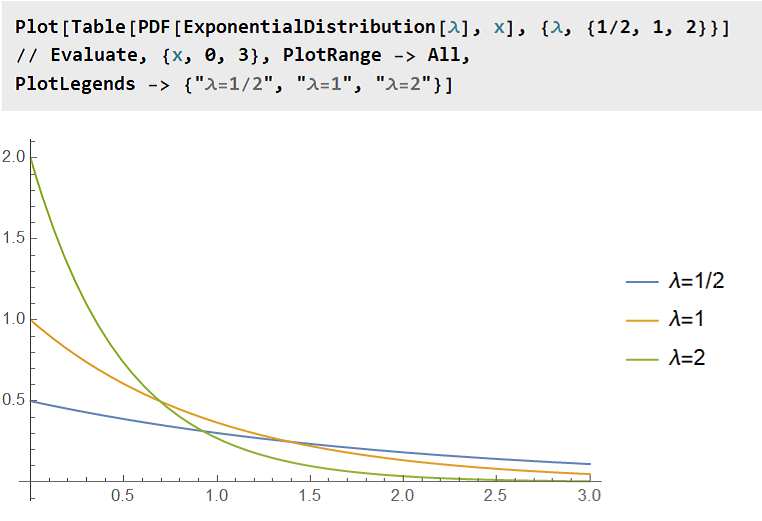
\includegraphics[scale=0.5]{plot.png}
\end{block}
\end{frame}

\begin{frame}{Exponential Distribution}
\begin{block}{Example}
$n$ light bulbs are burning simultaneously and independently, and the lifetime for each bulb follows the $\operatorname{Exp}(\beta)$.
\begin{itemize}
\item What is the distribution of the length of time $Y_{1}$ until the first failure in one of the $n$ bulbs?
\item What is the distribution of the length of time $Y_{2}$ after the first failure until a second bulb fails?
\end{itemize}
\end{block}
\pause
\begin{block}{Solution}
(i) Suppose random variables $X_{1}, \ldots, X_{n}$ satisfies that $X_{i} \sim \operatorname{Exp}(\beta)$, and $Y_{1}=\min \left\{X_{1}, \ldots, X_{n}\right\} .$ Then for any $t>0$,
$$
P\left[Y_{1}>t\right] =P\left[X_{1}>t, \ldots, X_{n}>t\right] 
$$
$$
=P\left[X_{1}>t\right] \times \cdots \times P\left[X_{n}>t\right] =e^{-n \beta t}
$$
indicating an exponential distribution with parameter $n \beta$.
\end{block}
\end{frame}

\begin{frame}{Exponential Distribution}
\begin{block}{Example}
$n$ light bulbs are burning simultaneously and independently, and the lifetime for each bulb follows the $\operatorname{Exp}(\beta)$.
\begin{itemize}
\item What is the distribution of the length of time $Y_{1}$ until the first failure in one of the $n$ bulbs?
\item What is the distribution of the length of time $Y_{2}$ after the first failure until a second bulb fails?
\end{itemize}
\end{block}
\begin{block}{Solution}
(ii) Exponential Distribution is memoryless.
$$
P\left[Y_{2}>t\right] =P\left[X_{2}>t, \ldots, X_{n}>t\right] 
$$
$$
=P\left[X_{2}>t\right] \times \cdots \times P\left[X_{n}>t\right] =e^{-(n-1) \beta t}
$$
indicating an exponential distribution with parameter $(n-1) \beta$.
\end{block}
\end{frame}


%%gamma
\begin{frame}{Gamma Distribution}
\begin{block}{Definition}
Let $\alpha, \beta \in \mathbb{R}, \alpha, \beta>0$. A continuous random variable $\left(X, f_{\alpha, \beta}\right)$ follows a gamma distribution with parameters $\alpha$ and $\beta$ if the probability density function is given by
$$
f_{\alpha, \beta}(x)= \begin{cases}\frac{\beta^{\alpha}}{\Gamma(\alpha)} x^{\alpha-1} e^{-\beta x}, & x>0 \\ 0, & x \leq 0\end{cases}
$$
\end{block}
where $\Gamma(\alpha)=\int_{0}^{\infty} z^{\alpha-1} e^{-z} \mathrm{~d} z, \alpha>0$ is the Euler gamma function.
Interpretation. 
\begin{block}{Interpretation}
The time needed for the next $r$ arrivals in a Poisson process with rate $\lambda$ follows a Gamma distribution with parameters $\alpha=r, \beta=\lambda$.
\end{block}
\end{frame}

\begin{frame}{Gamma Distribution}
\begin{block}{Properties}
\begin{itemize}
\item Mean.
$$
\mathrm{E}[X]=\frac{\alpha}{\beta}
$$
\item Variance. 
$$
\operatorname{Var}[X]=\frac{\alpha}{\beta^{2}}
$$
\item M.G.F.
$$
m_{X}:(-\infty, \beta) \rightarrow \mathbb{R}, \quad m_{X}(t)=\frac{1}{(1-t / \beta)^{\alpha}}
$$
\end{itemize}
\end{block}
\end{frame}


\begin{frame}{Gamma Distribution}
\begin{block}{Plot}
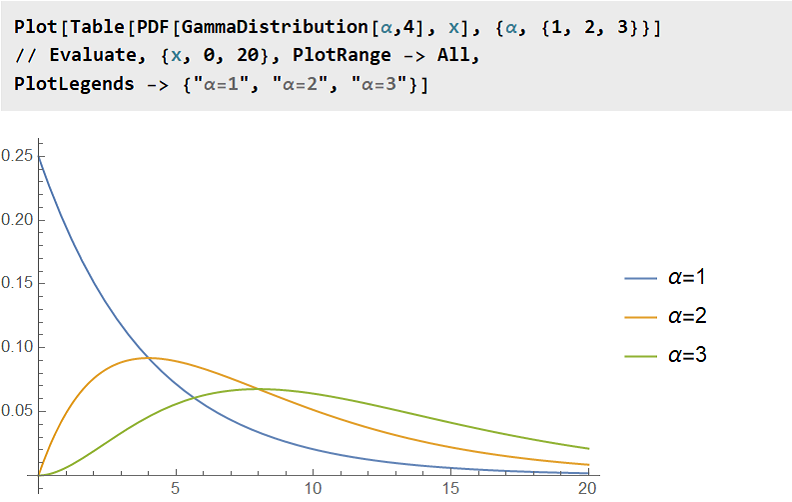
\includegraphics[scale=0.5]{gamma1.png}
\end{block}
\end{frame}

\begin{frame}{Gamma Distribution}
\begin{block}{Plot}
What's Wrong?
-- FOR $\beta$, MMA IS DIFFERENT FROM THE LECTURE! It's $(1/2,1/4,1/6)$ for the lecture version.

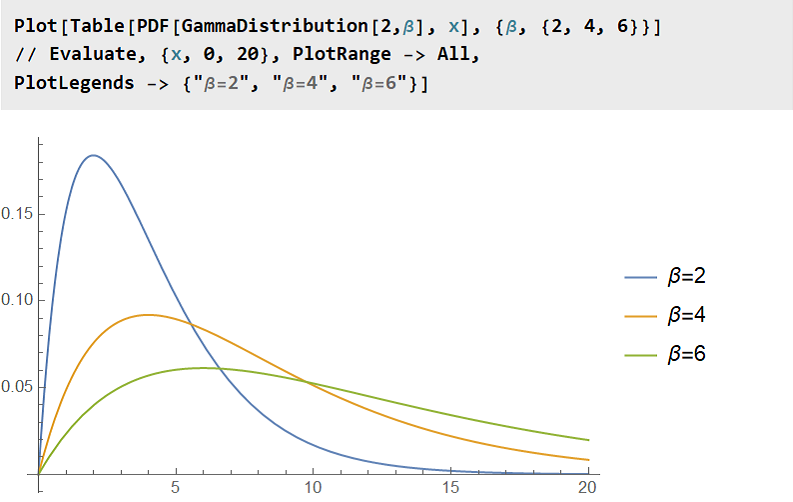
\includegraphics[scale=0.5]{gamma2.png}
\end{block}
\end{frame}

\begin{frame}{Chi-Squared Distribution}
\begin{block}{Definition}
Definition. Let $\gamma \in \mathbb{N}$. A continuous random variable $\left(X_{\gamma}^{2}, f_{X}\right)$ follows a chi-squared distribution with $\gamma$ degrees of freedom if the probability density function is given by
$$
f_{\gamma}(x)= \begin{cases}\frac{1}{2^{\gamma / 2} \Gamma(\gamma / 2)} x^{\gamma / 2-1} e^{-x / 2}, & x>0 \\ 0, & x \leq 0\end{cases}
$$
\end{block}
It is a gamma distribution with $\alpha=\gamma / 2, \beta=1 / 2$. Therefore,
$$
\mathrm{E}\left[X_{\gamma}^{2}\right]=\gamma, \quad \operatorname{Var}\left[X_{\gamma}^{2}\right]=2 \gamma
$$
\end{frame}

\begin{frame}{Chi-Squared Distribution}
\begin{block}{Plot}
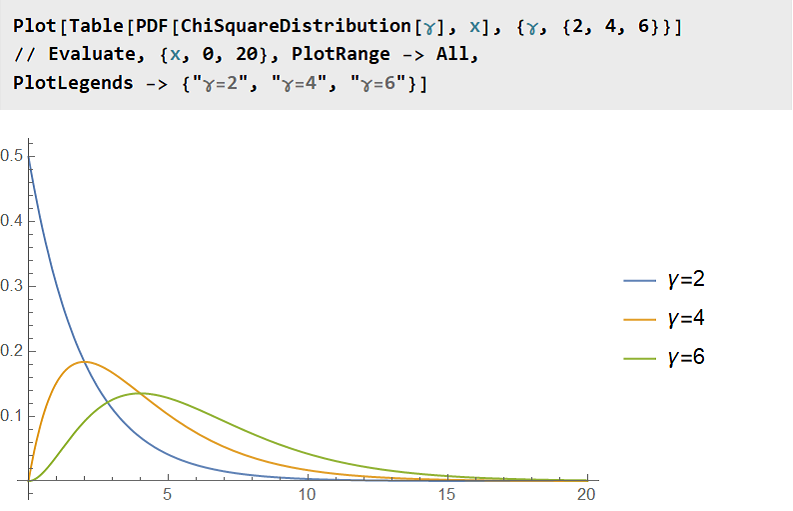
\includegraphics[scale=0.5]{chi.png}
\end{block}
\end{frame}


\section{Supplementary Materials}
\subsection{Exercise and Discussion}
\begin{frame}{1.Integral to Distribution}
\begin{block}{Exercise}
For $0<p<1$ and $n=2,3, \ldots$, determine the value of
$$
\sum_{x=2}^{n} x(x-1)\left(\begin{array}{l}
n \\
x
\end{array}\right) p^{x}(1-p)^{n-x}
$$
\end{block}
\end{frame}

\begin{frame}{2.Poisson Approximation to the Binomial}
\begin{block}{Discussion}
Prove that we can approximate the \bb{Binomial distribution} with \bb{Poisson distribution} when $n$ is large (Have Fun!).
\end{block}
\begin{block}{Exercise}
A factory produces drill bits. It is known that $2 \%$ of the drill bits are defective. The drill bits are shipped in packages of 100 . Use the Poisson approximation to the binomial distribution to answer the following questions.
\begin{enumerate}
\item What is the probability that there are no more than three defective drill bits in a package?
\item How many drill bits must a package contain so that with probability greater than $0.9$ there are at least 100 non-defective drill bits in the package?
\end{enumerate}
\end{block}
\end{frame}

\begin{frame}{3.Relationship Between Poisson and Exponential}
\begin{block}{Discussion}
Prove that the time between successive arrivals of a \bb{Poisson-distributed} random variable is \bb{exponentially distributed} with parameter $\beta=\lambda$.
\end{block}
\begin{block}{Exercise}
A certain widget has a mean time between failures of 24 hours, i.e., failures occur at a constant rate of one failure every 24 hours.

One evening, the widget was observed to be working at $10 \mathrm{pm}$ and then left unobserved for the night. The next morning at $6 \mathrm{am}$, it was observed to have failed earlier. What is the probability that it was still working at 5 am that morning?
\end{block}
\end{frame}

\begin{frame}{4.Stock Control Problem}
\begin{block}{Exercise}
To determine the level to which the stock of some commodity should be allowed to fall before an order for a new batch is placed. The general procedure is to choose this level so as to give a specified probability of a stockout before the new batch arrives. 

This probability $P_n$, known as the risk level, must hence be determined as a function of the reorder level $n$. It will, in fact, equal the probability that the number of demands during the lead time exceeds $n$.
\end{block}
\end{frame}
\begin{frame}{4.Stock Control Problem}
\begin{block}{Exercise}
We shall consider the two problems just described in the case where:
\begin{itemize}
\item The demand is random in the sense that the number of demands $r$ during a fixed interval of time $t$ has a Poisson distribution
$$
\frac{e^{-\lambda t}(\lambda t)^{r}}{\Gamma(r+1)}
$$
\item The lead time $t$ has a gamma type probability density function
$$
\frac{\mu e^{-\mu t}(\mu t)^{k-1}}{\Gamma(k)}
$$
With mean $\mathrm{k} / \mu$ and variance $\mathrm{k} / \mu^{2}$.
\end{itemize}
\end{block}
\end{frame}

\end{document}